\section{Netzplan}
Im folgenden Netzplan sind alle Arbeitspakete der Entwicklung des Avocado-Share dargestellt. 
Um sicherzustellen, dass jedes Arbeitspaket termingerecht und vollständig ausgeführt wird, haben wir beschlossen, neben dem Verantwortlichen auch eine Person zu bestimmen, welche eine Aufgabe ausführt.\\

Durch eine Planungsphase zu Beginn des Projektes, ist es uns möglich eine klare Schichtentrennung zu machen.
Da wir in der Planung die Schnittstellen zwischen den Schichten \todo{Wort fehlt},ist es uns möglich die Entwicklungsschritte danach
alle parallel auszuführen. Dadurch erhalten wir zwar einen kleinen Flaschenhals beim Erstellen der Grobstruktur und des
Grundgerüstes, doch es bringt uns viel Freiheit in den folgenden Paketen. So können wir besser und einfacher allfällige
Verzögerungen und Ausfälle reagieren.
Da wir eine technisch saubere Lösung haben wollen, ist es uns wichtig, dass die Spezialisten eines Bereiches in unserem Team auch entweder Verantwortlicher oder Ausführender eines Arbeitspaketes sind. \\

In jedem Arbeitspaket inbegriffen ist, wo möglich, auch das Testing.
Bei Arbeitspaketen in welchen Java-Code geschrieben wurde, sollten Unit-Tests geschrieben werden.
Bei Web- und UI-Paketen sollte ein kurzes Test-Protokoll geschrieben werden, um sicherzustellen, dass alle Funktionen auch korrekt funktionieren.
So kann beim Arbeitspaket Testing schnell und einfach alles nochmals getestet werden.\\

Design- und Planungspakete haben als "`Test"' ein Review mit dem gesamten Team.

\begin{landscape}
% \vspace*{\fill}: center vertically 
% source: https://stackoverflow.com/questions/3141702/vertically-centering-a-title-page
\vspace*{\fill}
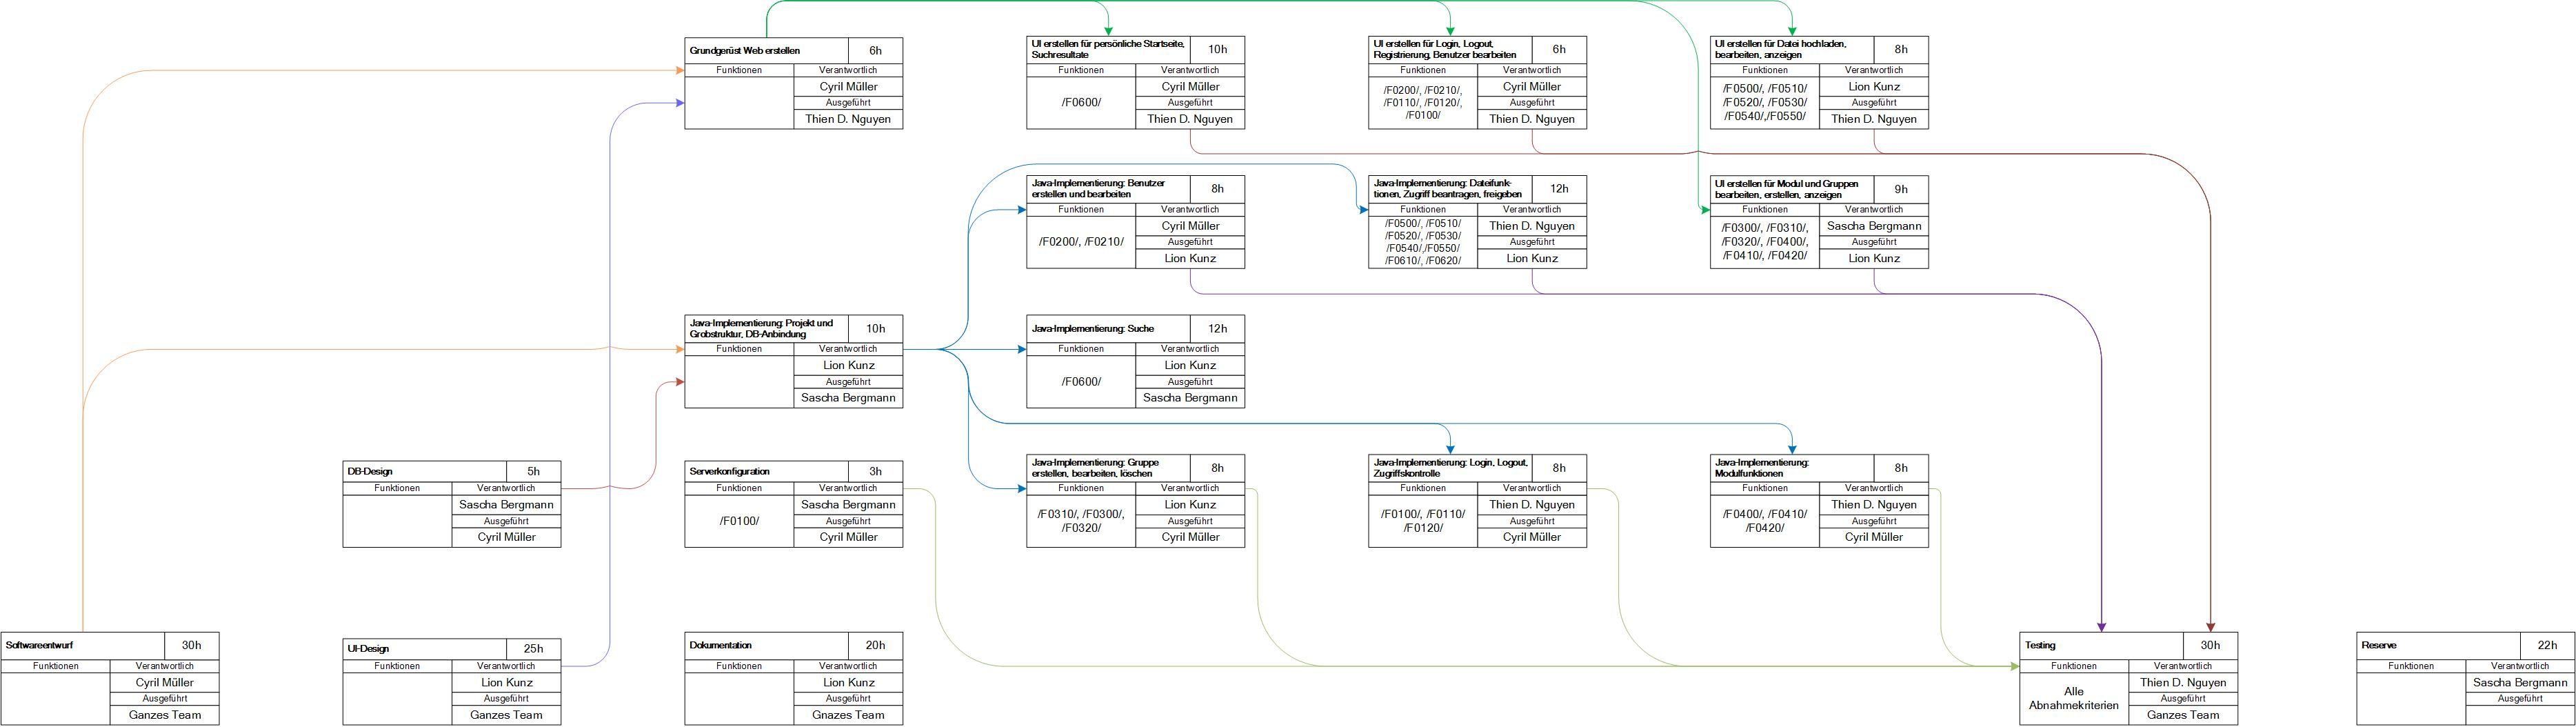
\includegraphics[width=\linewidth-1cm]{graphics/netzplan.jpg}
\vspace*{\fill}
\end{landscape}